\documentclass{article}
\usepackage{graphicx}

\date{August 7, 2017}
\title{Tutorial 1 - RW364}
\author{
  Ieuan, Uys\\
  \texttt{18218067@sun.ac.za}
}

\begin{document}
\maketitle

\section{Greenscreen}
The image was first seperated with a vectorized calculation of boolean arrays. The original image is split up into the color channels and then the values are compared to threshold values that were found to best remove the green screen background.



\begin{figure}[h!]
\centering
  \begin{minipage}[b]{0.3\textwidth}
    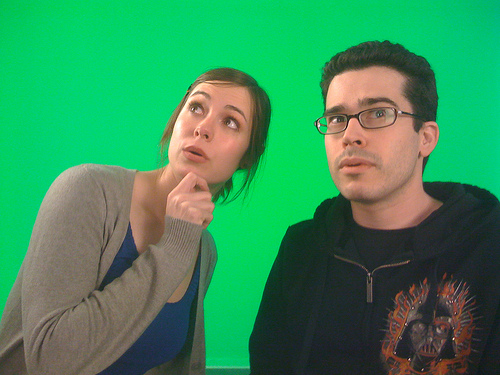
\includegraphics[width=\textwidth]{greenscreen.jpg}
    \caption{Greenscreen.png}
  \end{minipage}
  \hfill
  \begin{minipage}[b]{0.3\textwidth}
    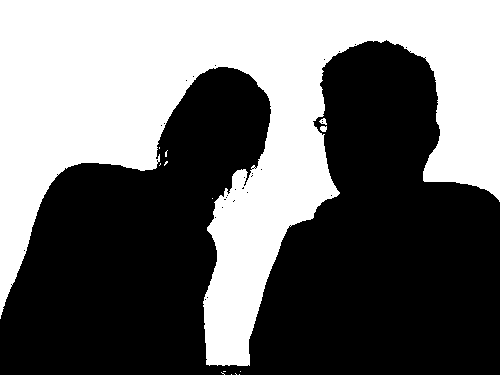
\includegraphics[width=\textwidth]{Q1_1.png}
    \caption{Threshold.png}
  \end{minipage}
  \hfill
  \begin{minipage}[b]{0.3\textwidth}
    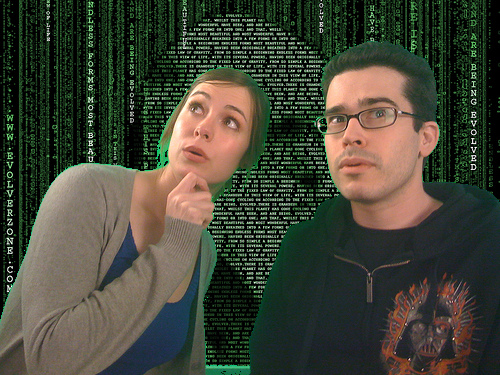
\includegraphics[width=\textwidth]{Q1_2.png}
    \caption{NewImage.png}
  \end{minipage}
\end{figure}


\section{Unsharp Mask}

The method of the unsharp mask is a simple one.\\
I began with a simple greyscale image.\\
See the entire transformation (Figure 4 - 5).

\begin{figure}[h!]
\centering
  \begin{minipage}[b]{0.45\textwidth}
    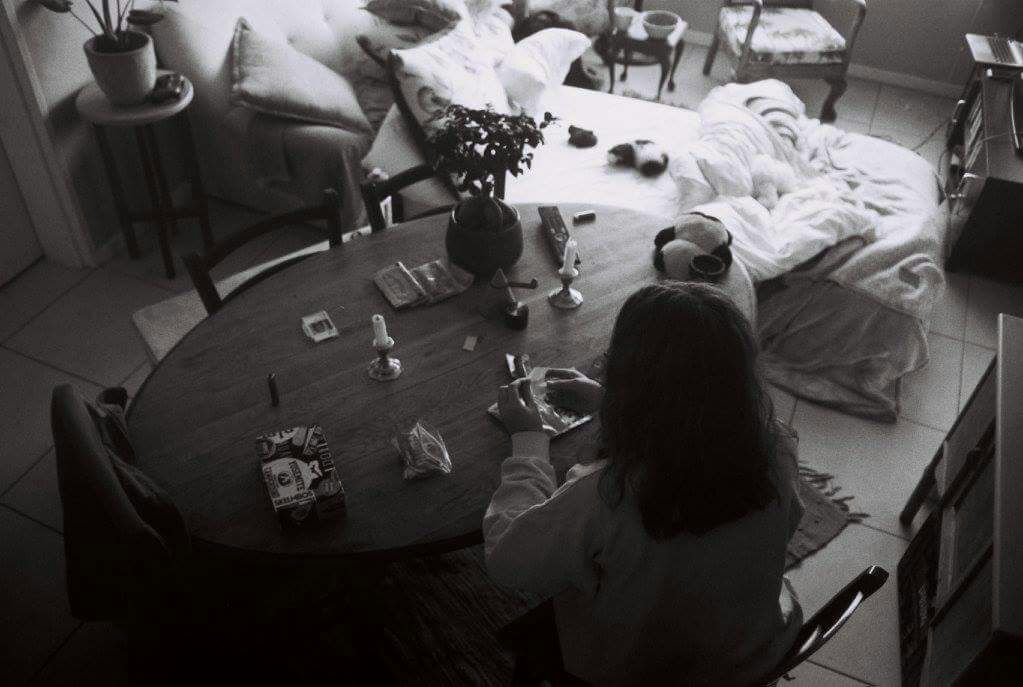
\includegraphics[width=\textwidth]{Q2.jpg}
    \caption{Image before any effects}
  \end{minipage}
  \hfill
  \begin{minipage}[b]{0.45\textwidth}
    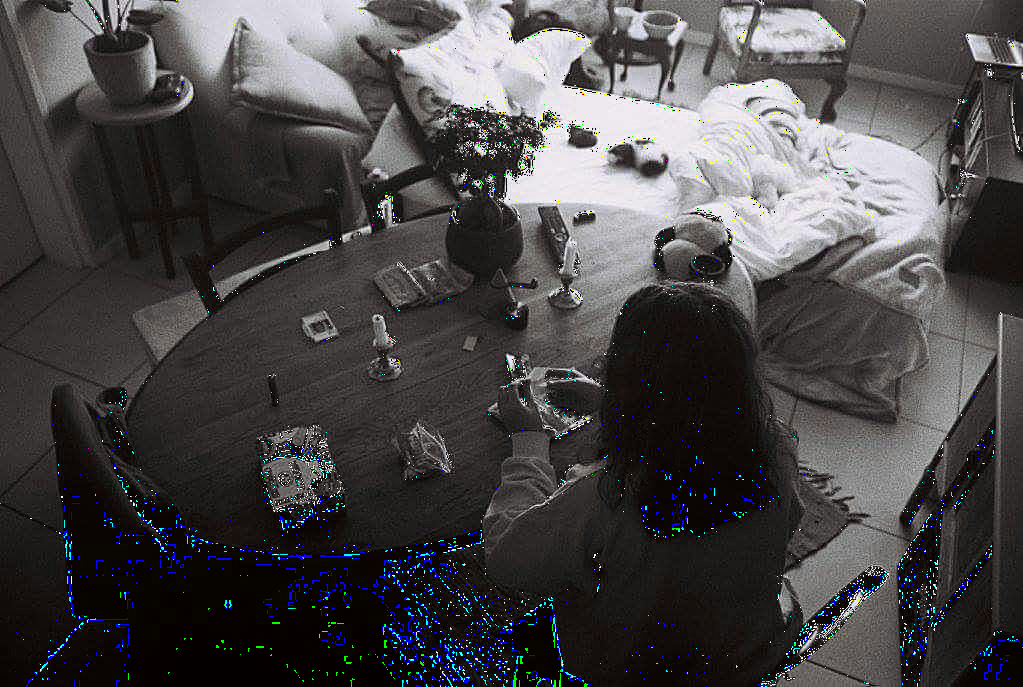
\includegraphics[width=\textwidth]{Q2_fin.png}
    \caption{Final image after effects}
  \end{minipage}
 \end{figure}

Between steps it is neccesary to blur and take the difference of the blur and the initial image.
\\See Figure 6 \& 7.

\begin{figure}[h!]
\centering
  \begin{minipage}[b]{0.45\textwidth}
    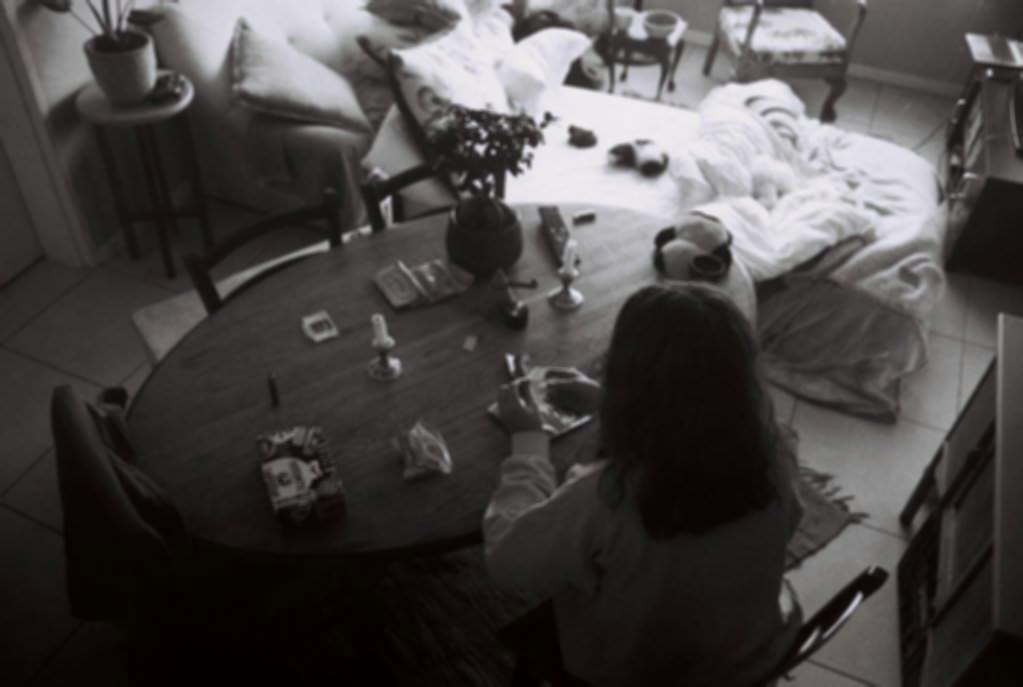
\includegraphics[width=\textwidth]{Q2_blur.png}
    \caption{Apply Gaussian blur}
  \end{minipage}
  \hfill
  \begin{minipage}[b]{0.45\textwidth}
    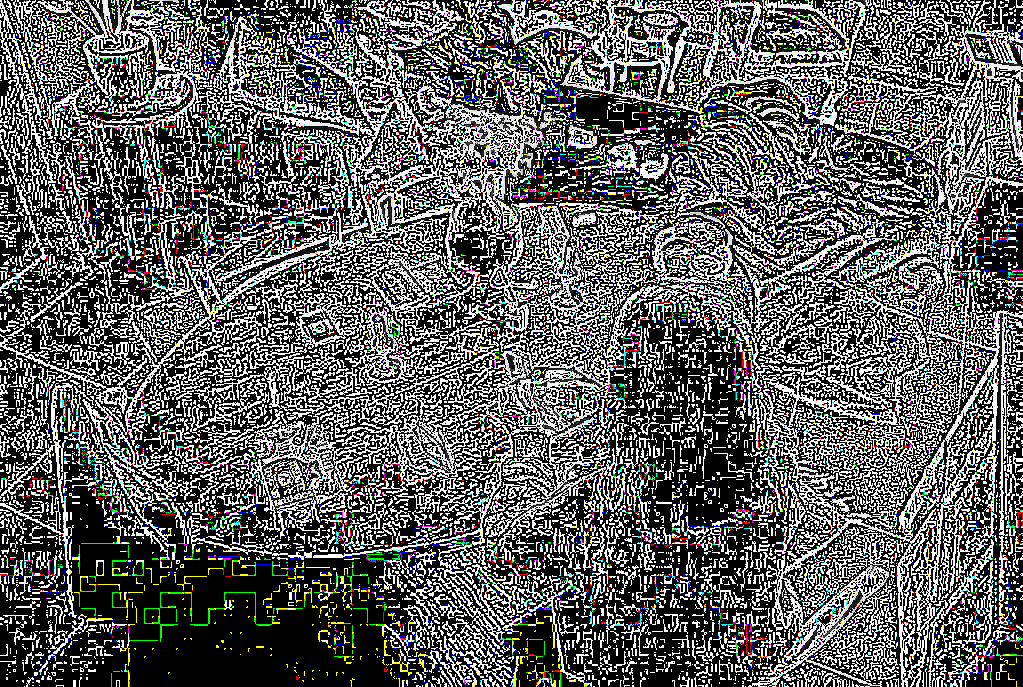
\includegraphics[width=\textwidth]{Q2_diff.png}
    \caption{difference of (4) and (6)}
  \end{minipage}
\end{figure}

To compare my sharpened image I used the openCV library to make a second unsharped mask and this is what you see compared bellow.

\begin{figure}[h!]
\centering
  \begin{minipage}[b]{0.45\textwidth}
    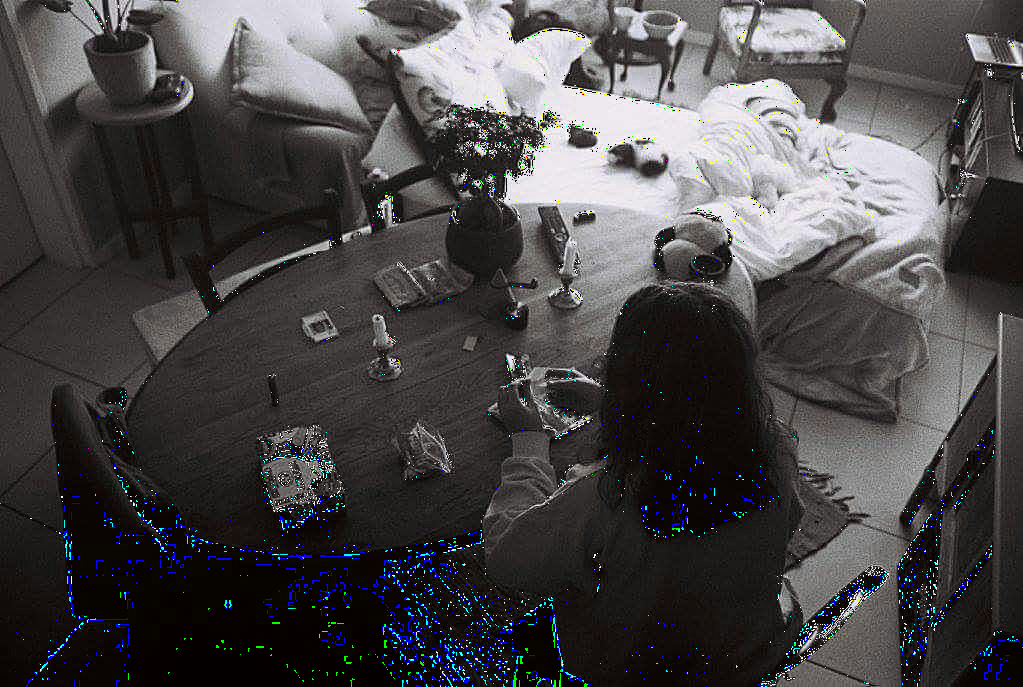
\includegraphics[width=\textwidth]{Q2_fin.png}
    \caption{My Unsharp Mask}
  \end{minipage}
  \hfill
  \begin{minipage}[b]{0.45\textwidth}
    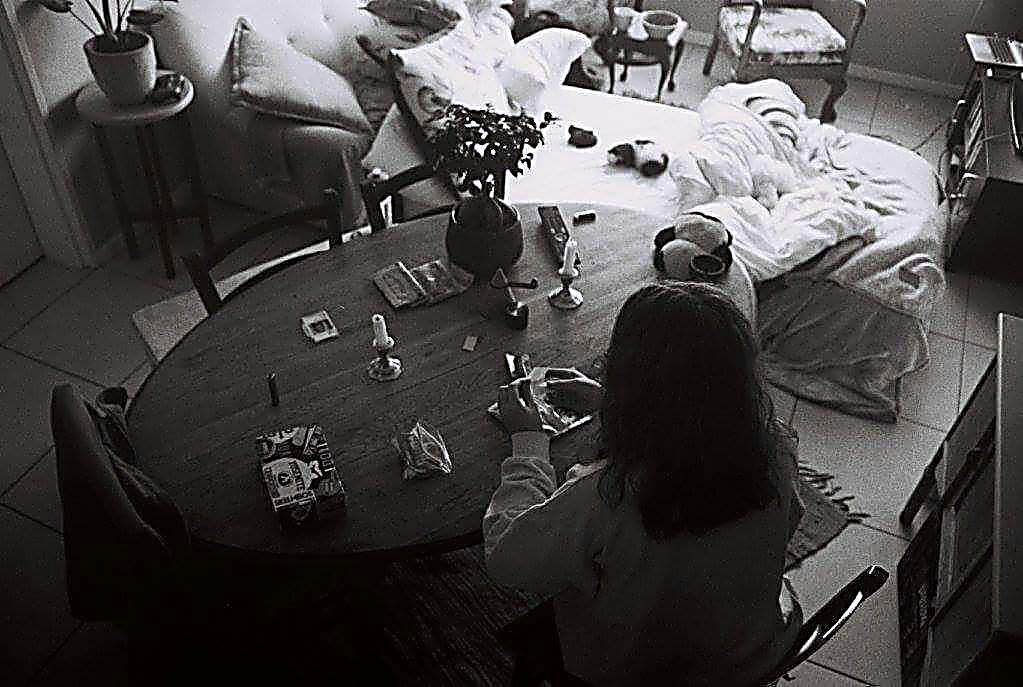
\includegraphics[width=\textwidth]{Q2_cv2.png}
    \caption{openCV library}
  \end{minipage}
\end{figure}

\subsection{Overflow}
As you can clearly see, there are many pixels with rgb values outside of the range of [0, 255] which results in bogus image data. This is caused by the mathematics behind the method of unsharp masking and is a normal result. I have also added a unsharp mask implemented by the openCV library which has made provision for the case. I believe that it would be better to scale all the intensities to set the highest overflow value to 255 and the lowest underflow values to 0 so as to maintain the contrast.

\section{Image Scaling}
Resizing of images is made simple through inverse transformation, here are examples of my Nearest Neighbour and Bilinear implementations.

\subsection{Nearest Neighbour}
The nearest neighbour makes use of very simple rounding to interpolate the pixels in the new rescaled image. See figure 11 \& 12.

\begin{figure}[h!]
\centering
  \begin{minipage}[b]{0.45\textwidth}
    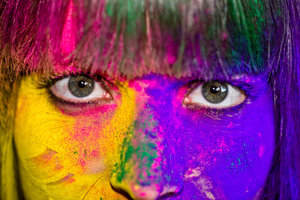
\includegraphics[width=\textwidth]{colour.jpg}
    \caption{The Original Image}
  \end{minipage}
  \hfill
  \begin{minipage}[b]{0.45\textwidth}
    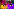
\includegraphics[width=\textwidth]{NN_0_05.png}
    \caption{NN with scale 0.5}
  \end{minipage}
\end{figure}

\subsection{Bilinear Interpolation}
The bilinear interpolation makes use of 4 samples when doing the inverse transformation to find the values of the color tuples in the new resized image.

\begin{figure}[h!]
\centering
  \begin{minipage}[b]{0.45\textwidth}
    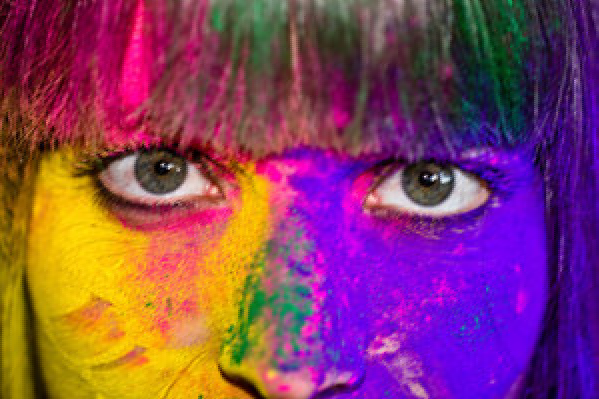
\includegraphics[width=\textwidth]{BI_2.png}
    \caption{BI with scale 2}
  \end{minipage}
  \hfill
  \begin{minipage}[b]{0.45\textwidth}
    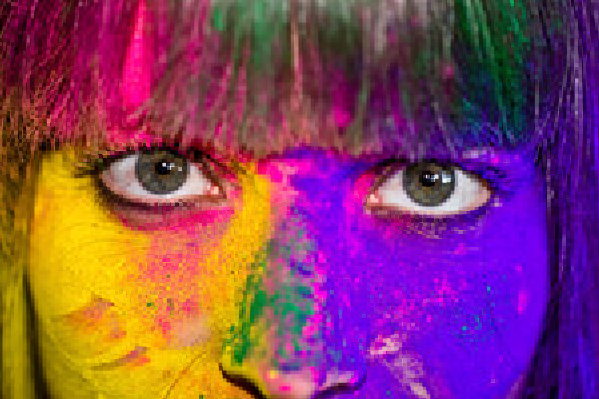
\includegraphics[width=\textwidth]{NN_2.png}
    \caption{NN with scale 2}
  \end{minipage}
\end{figure}


\subsection{Comparison}
When looking at Figure 14 and 15, which are zoomed versions of figure 12 \& 13, it is clear to see that the bilinear interpolation achives much better results than the nearest neighbour interpolation. In Figure 14 the edges are smoother and the eyelashes in the image are visible as opposed to figure 15 where the eyelashes are a large mass of pixels.

\begin{figure}[h!]
\centering
  \begin{minipage}[b]{0.45\textwidth}
    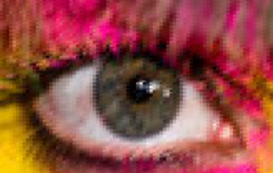
\includegraphics[width=\textwidth]{BI_2_zoom.png}
    \caption{BI with scale 2}
  \end{minipage}
  \hfill
  \begin{minipage}[b]{0.45\textwidth}
    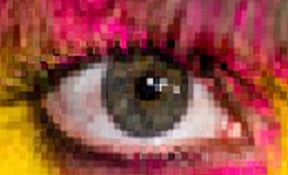
\includegraphics[width=\textwidth]{NN_2_zoom.png}
    \caption{NN with scale 2}
  \end{minipage}
\end{figure}

\section{Feature Detection}
I incurred errors in the section and was not able to implement Feature Detection nor was I able to complete Question 5

\section{Libraries}
\begin{itemize}
  \item matplotlib
  \item skimage
  \item numpy
  \item scipy
  \item math
  \item cv2
\end{itemize}

\end{document}
